\chapter{Marco teórico y estado del arte}
%% leer https://www.cd-genomics.com/blog/introduce-to-16s-rrna-and-16s-rrna-sequencing/

Esta tesis busca presentar una nueva alternativa para la caracterización de comunidades microbianas utilizando secuenciación de tercera generación. Para ello se  desarrolló un flujo de trabajo automatizado que permite realizar el procesamiento de los datos de secuenciación (control de calidad, asignación taxonómica, análisis de diversidad, predicción funcional y caracterización de grupos). 

Debido a que la ejecución de pipelines bioinformaticos requiere conocimiento de línea de comando y contar con recursos computacionales, se desarrolló una aplicación que permite al usuario abstraerse del conocimiento computacional requerido al analizar datos. Una vez que el usuario sube sus datos a la plataforma web, ésta envia los datos, ejecuta el flujo de trabajo y presenta los resultados en forma de gráficos y tablas en la plataforma.

% Para usar la plataforma el usuario debe llenar un formulario con la metadata de la secuenciación, subir los archivos e indicar los análisis a realizar, con esto la plataforma web enviará los datos de secuenciación a la plataforma de alto rendimiento y ejectará el flujo de trabajo, una vez finalizado, los resultados se presentarán en la plataforma web.

A continación se presenta el marco teórico y estado del arte de los conceptos necesarios para el desarrollo de esta tesis, como qué es la microbiota, el gen 16S rRNA, tecnologías de secuenciación y sus usos, las diferentes herramientas bioinformáticas para el análisis de datos y herramientas para el desarrollo de la aplicación web.
\section{Estudio de microbiota a traves del gen 16S y tecnologías de secuenciacion}
\subsection{Microbiota}
La microbiota es el conjunto de microorganismos (bacterias, virus, arqueas, u hongos) que habitan en un ambiente, ya sea en organismos multicelulares como humanos~\cite{gilbert2018current}, animales~\cite{bahrndorff2016microbiome} o plantas~\cite{berendsen2012rhizosphere}, y también en ambientes naturales como el océano~\cite{doi:10.1126/science.aac8455} y el suelo~\cite{banerjee2023soil}. 
Estos organismos que componen la microbiota se encuentran en un estado de simbiosis junto con el huesped, contribuyendo en funciones vitales como la homeostasis, regulación del sistema inmune, digestión de alimentos, producción de vitaminas, protección ante enfermedades y agentes patógenos~\cite{marco2021defining,fijan2014microorganisms,altvecs2020interaction,hou2022microbiota}. 
Sin embargo, una disbiosis o una baja diversidad en la microbiota se puede asociar a una desregulación en el organismo huesped, incluyendo diversos tipos de enfermedades, fallas en el sistema inmune, falta de vitaminas, trastornos como depresión, estrés, e incluso diferentes tipos de cáncer en el caso del ser humano~\cite{altvecs2020interaction,hou2022microbiota}.

La composición de la microbiota va cambiando dependiendo del área de estudio, pudiéndose encontrar diferentes microorganismos en las cavidades orales, zonas intestinales, genitales, cutáneas o tracto respiratorio~\cite{ursell2012interpersonal}.

%Se estima que en el ser humano habitan más de 10 billones de microorganismos~\cite{sender2016revised}, es decir, poseemos cerca de 350 billones de celulas microbioanas~\cite{fijan2014microorganisms,ley2006ecological} , siendo este número al menos 10 veces mayor que el número de células humanas que poseemos.

En la naturaleza los microorganismos cumplen un rol fundamental en los ciclos bioquímicos del nitrógeno, carbono y fósforo~\cite{bitton1994role, gougoulias2014role}, como también en los procesos de desnitrificación, nitrificación y mineralización~\cite{bitton1994role, gougoulias2014role}. 
Dependiendo del tipo de ambiente, los microorganismos también varian, en el caso del suelo por ejemplo, cambian dependiendo del tipo de suelo en el que están (agrícolas, forestales, humedales, pastos o suelos desérticos~\cite{jiao2021linking}) y de las características de éste como la temperatura, hidaratación, profundidad, cantidad de carbono~\cite{bickel2020soil}.
En el caso de las plantas, se ha demostrado que la microbiota presente ayuda a la adquisición de nutrientes~\cite{hu2017probiotic}, crecimiento, salud y resistencia a enfermedaddes~\cite{lemanceau2017let,hardoim2015hidden,vorholt2012microbial,COMPANT201929}.


La microbiota humana se puede ver afectada por diferentes factores, como los hábitos alimenticios, estilo de vida, uso de antibióticos, edad, estrés, entre otros~\cite{altvecs2020interaction}. 
La interacción con el medio ambiente también influye, habiendo estudios que identifican cambios en la microbiota de recién nacidos, infantes y adultos que viven con animales~\cite{tun2017exposure, azad2013infant,kates2020household}, como también cambios en la microbiota intestinal y cutánea en niños que interactuan con la naturaleza, plantas o suelo, identificando aumento en las vías inmunoreguladoras en comunidades microbianas cercanas a la naturaleza~\cite{roslund2020biodiversity}.

% https://www.frontiersin.org/articles/10.3389/fcimb.2012.00104/full?portfolio-raia-drogasil=1


% Microbiota: Microorganismos vivos encontrados en un ambiente definido (como por ejmplo en los tejidos orales o intestinales)

% microbioma: Colección de genomas de todos estos microorganismos en el ambiente (no solo las comunidades, elementos de su estructura microbial, metabolitos.)
Conocer la diversidad microbiana asociada a organismos multicelulares permite ahondar en la relación existente entre microbios y la salud de los seres vivos, asi como conocer microorganismos patógenos que causan enfermedades infecciosas, ayuda al diagnóstico y permite tomar acciones oportunas. 
Este conocimiento ayuda modular nutrición, salud y enfermedad a través del estudio del microbioma tomando en consideración los distintos factores asociados al estilo de vida.
% https://www.ncbi.nlm.nih.gov/pmc/articles/PMC6009232/
\subsection{ARN Ribosomal 16S}
%% seleccion region
%% https://search.brave.com/search?q=16s+gene+what+are+constant+and+variables+reigon&source=desktop
El ARN ribosomal 16S es un gen perteneciente a la subunidad menor 30S que codifica el rRNA bacteriano y se encuentra en todas las bacterías. 
Esta compuesto por 1542 pares de bases aproximadamente, divididas en 9 regiones hipervariables entrelazadas con regiones constantes~\cite{clarridge2004impact}.
Las regiones constantes son compartidas por todas las bacterias, mientras las regiones variables presentan cierto grado de variabilidad entre las especies. 


%%https://www.elsevier.es/es-revista-enfermedades-infecciosas-microbiologia-clinica-28-articulo-identificacion-bacteriana-mediante-secuenciacion-del-13059055#:~:text=El%20ARN%20ribos%C3%B3mico%20(ARNr)%2016S,la%20d%C3%A9cada%20de%2019702.

%El gen 16S rRNA esta compuesto de aproximadamente 1542 pares de bases divididas en 10 regiones conservadas y 9 regiones hipervariables.%, las cuales permiten llevar a cabo la  identificación de los organismos. 
\begin{figure}[H]
    \centering
    
\includegraphics[width=1\linewidth]{images/16s_diagram-2.pdf}
    \caption{Estructura de las regiones constantes e hipervariables del gen 16S rRNA}
    \label{fig:16S_structure}
\end{figure}
% \begin{figure}[H]
%     \centering
%     \includegraphics[width=1\linewidth]{images/16S_2.png}
%     \caption{Estructura de las regiones variables e hipervariables del gen 16S rRNA}
%     \label{fig:16S_structure2}
% \end{figure}


El uso de la macromolécula del ARN ribosomal  16S para el estudio de relaciones filogenéticas y de bacterias fue propuesto por Carl Woese a principios de 1970~\cite{olsen1993ribosomal}.
Sus caracteristicas únicas como su presencia en todas las bacterias, su alto grado de conservación (debido a que su función no cambia a través del tiempo) y su tamaño (el cuál permite ser lo suficientemente largo y preciso para la asignación taxónomica, y abordable para análisis bioinformáticos) hacen que hoy en día sea el marcador molecular más utilizado para la identificación de bacterias y comunidades microbianas~\cite{reller2007detection,janda200716s,lopez2023determining,patel200116s}.


Las regiones variables permiten llevar a cabo la caracterización de los microorganismos, siendo la metodología más utilizada el secuenciar parcialmente el gen 16S, es decir, secuenciar una o dos regiones y realizar la asignación taxónomica en base a la región secuenciada. Diversos estudios se han llevado a cabo para determinar los efectos de la selección de la región a utilizar para la identificación, llegandose a determinar que la región hipervariable ha secuenciar influye en los resultados de la comunidad y en la diversidad de microorganismos que se caracteriza~\cite{klindworth2013evaluation,mizrahi2013taxonomic,guo2013taxonomic,soergel2012selection}.

%\hl{Evaluation of general 16S ribosomal RNA gene PCR primers for classical and next-generation sequencing-based diversity studies} \hl{The impact of DNA polymerase and number of rounds of amplification in PCR on 16S rRNA gene sequence data, mSphere, vol. 4, 2019}



El gold standard para la identifición de bacterias durante muchos años fue el cultivo convencional en laboratorio, sin embargo, el cultivo puede durar desde días a semanas o incluso meses, y en algunos casos, hay bacterias que no se logran cultivar en laboratorio~\cite{didelot2012transforming}. 
Es por esto, que las tecnologías de secuenciación de nueva generación se presentaron como una buena alternativa y se empezaron a usar masivamente para secuenciar el gen 16S y caracterizar comunidades al permitir secuenciar comunidades complejas (y no solo aislados) y al permitir secuenciar millones de lecturas al mismo tiempo~\cite{reller2007detection}, haciendo que la forma de caracterizar bacterias sea más estándar y abordable al día de hoy~\cite{woo2008then, tanner1994impact}. 
%El estudio de comunidades microbianas mediante el gen 16S rRNA se ha vuelto una herramienta poderosa tanto en ambientes clínicos como ambientales, permitiendo obtener información de la diversidad de una muestra de manera más rápida y económica que con los métodos tradicionales~\cite{buscar}.
%Las tecnologías de secuenciación  permiten la identificación de bacterias a través de  \hl{signatures/firmas} únicas 

%Existen diferentes bases de datos que contienen la información de las secuencias del gen 16S para las diferentes bacterias, como 16S en bases de datos como RDP (Ribosomal Database Project~\cite{cole2014ribosomal}), 16S RefSeq~\cite{}, Greengenes~\cite{desantis2006greengenes}, Silva~\cite{} y el proyecto de microbioma humano (HMP)~\cite{}.



%añadir: GEN 16S RRNA ES el gold standar para analisis filogeneticos~\cite{boers2019understanding}.

%Las regiones constantes se utilizan para el diseño de primers a utilizar durante la amplificación (PCR), LAS REGIONES hipervariales se utilizan para la identificación de diversidad en procariontes~\cite{chakravorty2007detailed}.
\subsection{Secuenciación de ADN}
Todo ser vivo cuenta con una molécula de ADN que contiene la información genética del individuo. Ésta información se códifica a través de bases nitrogenadas: adenina (A),timina (T), guanina (G) y citosina (C)~\cite{watson1953molecular}. 
Para determinar esta secuencia de nucleótidos se han desarrollado diferentes técnicas las que se conocen como secuenciación de ADN. 

Las tecnologías de secuenciación se pueden dividir en tres generaciones, cada una con diferentes características, como los largos de las moleculas a secuenciar, porcentaje de error, costo y cantidad de información que secuencian (\textit{throughput}).
Las tecnologías de secuenciación de nueva generación (NGS) involucran las tecnologías de segunda y tercera generación (short-reads y long-reads respectivamente) y se diferencian de la primera generación de secuenciación por la cantidad de información que permiten obtener en la secuenciación, y por haber reducido notablemente los costos y tiempos de secuenciación, pero presentando un porcentaje de error mayor~\cite{kumar2024next}. 

Independiente de la tecnología de secuenciación a utilizar, el proceso de secuenciación de ADN se puede dividir en tres etapas: preparación de librería, secuenciación y análisis de las datos. Durante la preparación de las librerias el ADN se fragmenta en tamaños manejables para el secuenciador que luego son secuenciados. El resultado de la secuenciación es un conjunto de secuencias de nucleótidos conocidas como \textit{read} o lectura.
Debido a las diferentes caracterisitcas de cada generación, al analizar las secuencias los análisis bioinformáticos y herramientas a utilizar también cambian dependiendo principalmente de la precisión del secuenciador utilizado y el tamaño de las lecturas producidas~\cite{bierman2014understanding}.

%La precisión de estas tecnologías se puede medir mediante la precisión de la lectura raw (precisión al leer un sólo fragmento de ácido nucleico a la vez) o la precisión de los ensamblajes mediante consensos (reconstrucción de genomas completos).

La Figura \ref{fig:DNA_sequencing} presenta una comparativa entre las principales tecnologías de secuenciación de ADN, mostrando las diferencias entre las tecnologías de primera, segunda y tercera generación. En las siguientes secciones se detalla el funcionamiento de cada tecnología y sus caracteristicas más importantes.
\begin{figure}[H]
    \centering
    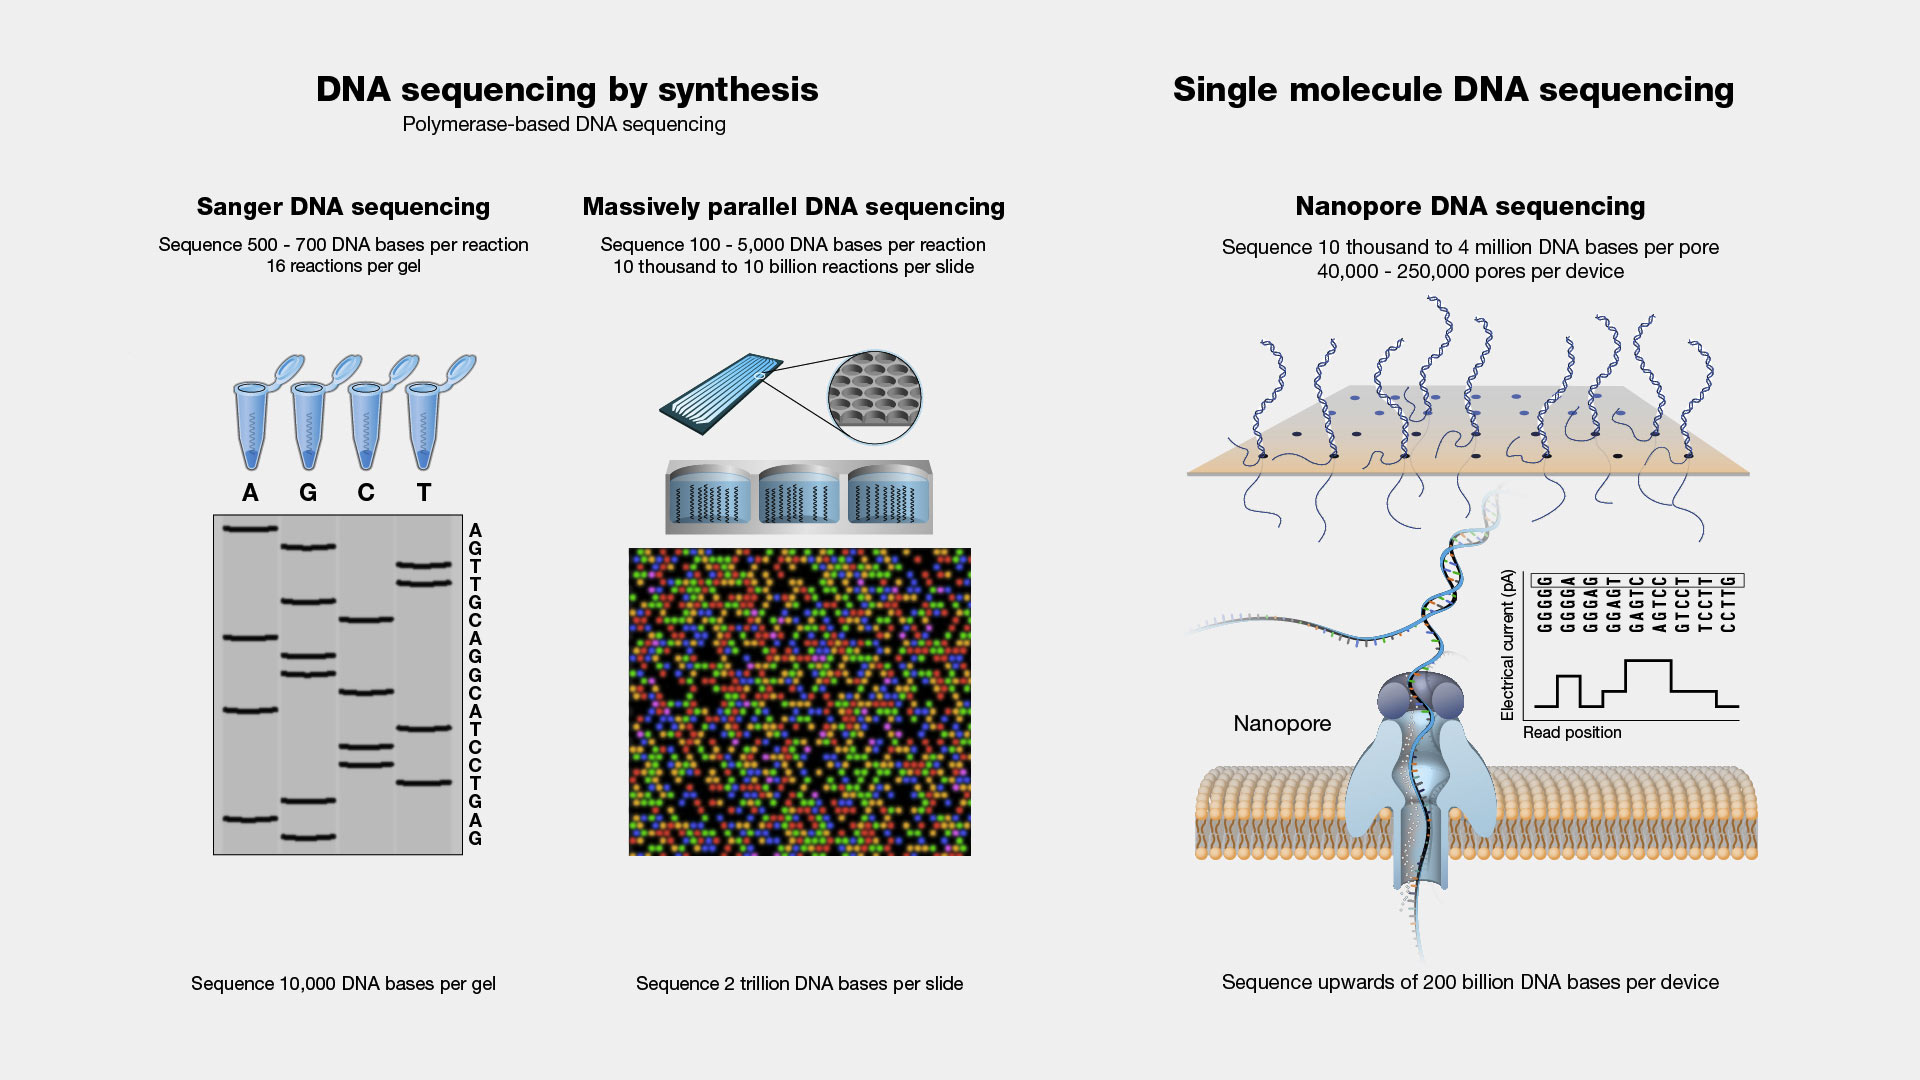
\includegraphics[width=1\linewidth]{images/DNA-Sequencing.jpg}
    \caption[Comparativa tecnologías de secuenciación]{Comparativa tecnologías de secuenciación de ADN\protect\footnotemark.}
    \label{fig:DNA_sequencing}
\end{figure}
\footnotetext{Fuente: https://www.genome.gov/genetics-glossary/DNA-Sequencing}
\subsubsection{Primera generación: Sanger}
Frederick Sanger introdujó la primera generación de tecnologías de secuenciación en el año 1977. El método Sanger utiliza el principio de ``terminación de cadena'' para secuenciar material genético~\cite{sanger1975rapid}. 
%Esta técnica replica el ADN utilizan nucleotidos modificados marcados con fluorescencia que detienen el proceso de replicación.
Durante la PCR se añaden nucleótidos modificados (ddNTPs) marcados con fluoroforo que al ser incorporados en la cadena de ADN detienen la elongación de ésta. Una vez que la reacción ha terminado, se realiza una electroforesis capilar que separa las moleculas de ADN por tamaño y con alta resolución para poder determinar la secuencia de la cadena, generando una única secuencia de como máximo 800 pares de bases por corrida~\cite{crossley2020guidelines}.

La principal ventaja de este método es su alta precisión (99.999\%), siendo ampliamente utilizado en diagnóstico clínico para la detección de mutaciones puntuales. Además de no requerir capacidad de cómputo ni conocimientos bioinformáticos para la generación de la secuencia.  
Entre sus principales desventajas se encuentras que es un método laborioso, costoso e ineficiente al trabajar en proyectos de secuenciación de gran escala como por ejemplo genomas completos o metagenómica debido a la cantidad de información que se puede obtener en la secuenciación, ya que permite obtener una sola secuencia por corrida.
 
Debido a su alta precisión, al secuenciar el gen 16S con Sanger se permite la caracterización a nivel de especie, pero también se pueden encontrar algunas limitantes, como por ejemplo que esta técnica permite detectar una sola especie a la vez. En caso de tener una muestra aislada, la secuenciación permitirá determinar la especie asociada al aíslado, pero en el caso de que la muestra presente más de una bacteria, la señal que se obtendra será una mezcla de las diferentes bacterias, por lo que será imposible realizar una caracterización. 
Esto limita su uso en comunidades complejas o infecciones polibacterianas ~\cite{lamoureux2022prospective}, donde para identificar la comunidad se deben usar tecnologías de secuenciación de nueva generación.
\subsubsection{Segunda generación: Secuenciación de lecturas cortas}
Las tecnologías de secuenciación de segunda generación más importantes son Illumina, IonTorrent y Roche 454. Éstas utilizan el principio de síntesis de cadena complementaria y una señal asociada al nucleótido incorporado (que puede ser fluorescencia, iones cargados, entre otros). %al unirse con la hebra complementaria. 
Esta generación de secuenciadores se caracteriza por ser rápida, de bajo costo, y por permitir obtener simultaneamente millones de moleculas de ADN mediante amplificación clonal o \textit{bridge} PCR, generado en paralelo millones de fragmentos cortos de ADN, de entre 35 a 600 pares de bases, con una precisión de 99.9\%.%, mediante una secuenciación rápida y de bajo costo~\cite{kumar2024next}.


Las principales metodologías de secuenciación de segunda generación son secuenciación por síntesis, utilizada principalmente por Illumina, y secuenciación por ligación utilizada por Roche 454~\cite{mardis2008next}.
Illumina es la \textit{NGS} más utilizada para la secuenciación del gen 16S. Este método utiliza secuenciación por síntesis: la primera etapa corresponde a la fragmentación de ADN y ligación de adaptadores.
Luego los fragmentos de ADN se unen a la superficie de la celda y se amplifican localmente para formar clusters. 
En cada ciclo de secuenciación se añaden nucleótidos marcados con fluoróforos que son removidos para continuar con el siguiente ciclo.
Finalmente, el secuenciador detecta la señal de fluorescencia y registra la secuencia de nucleótidos. 
Illumina posee diferentes dispositivos de secuenciación que permiten obtener \textit{reads} de 2x150 a 2x300 pares de bases como máximo.

Algunas de las plataformas de secuenciación de segunda generación utilizan secuenciación \textit{pair-end} donde cada fragmento de ADN se secuencia en ambas direcciones,  lo que permite obtener fragmentos de mayor tamaño mediante el solapamento de ambas lecturas. 

Dentro de las principales ventajas de las tecnologías de lecturas cortas se encuentra su bajo porcentaje de error, bajo costo, y la gran cantidad de herramientas bioinformáticas ya desarrolladas para trabajar con este tipo de datos~\cite{heather2016sequence}. Por otro lado, el tamaño de los fragmentos secuenciados es su mayor limitante, haciendo más compleja o imposible la resolución de regiones repetitivas o análisis más complejos como el ensamblaje de genomas.


La caracterización de comunidades microbianas con Illumina se ha convertido en el estándar, debido a su bajo costo,througput y alta precisión. Sin embargo las tecnologías de lecturas cortas permiten secuenciar solo una parte del gen 16S rRNA, debido al tamaño de las moleculas que secuencian (lecturas de entre 200 a 400pb)~\cite{salipante2014performance}. 
Diversos estudios se han realizado para analizar qué región permite obtener la mayor diversidad posible y de manera más precisa~\cite{liu2008accurate,schloss2011reducing}. También se ha determinado que existen grupos taxonómicos que se identifican de mejor manera al utilizar cierta regiones hipervariables~\cite{he2013comparison,claesson2010comparison}. De igual forma se ha determinado que al realizar una secuenciación parcial del gen 16S la resolución taxonómica es menor, llegandose a identificar solo hasta el nivel de género~\cite{liu2008accurate}.
 
Es por esto, que las tecnologías de tercera generación, Oxford Nanopore y PacBio se presentan como opciones prometedoras para la secuenciación del gen 16S rRNA, debido a su bajo costo y su capacidad de secuenciar el gen completo en un solo \textit{read}, lo que permite una mayor resolución taxonómica a nivel de especie o incluso de cepa~\cite{szoboszlay2023nanopore,10.1186/s13742}.%~\cite{urban2021freshwater,delahaye2021sequencing}. \hl{revisar estas citas}

%-----------------


%https://sampled.com/short-read-sequencing-vs-long-read-sequencing/#:~:text=Short%2Dread%20sequencing%2C%20as%20the,these%20pieces%20through%20a%20sequencer.

%Al secuenciar el gen 16S con Illumina se sabe que existe presencia de ruido, por lo que se deben realizar filtros como la eliminación de quimeras, eliminación de secuencias singleton y otus raros~\cite{caporaso2011global,auer2017analysis}, realizar denoising con dada~\cite{callahan2016dada2} y unoise~\cite{edgar2016unoise2}. Todas estos filtros y metodologias de trabajo no están disponibles para usarse con TGS como Nanopore y PacBio, debido al porcentaje de error y al tamaño de las lecturas.
%Mientras algunos estudios han demostrado, que Nanopore presenta un porcentaje de ruido muy bajo, casi nulo~\cite{szoboszlay2023nanopore}, y a su vez, al secuenciar el gen completo, y no contar con OTUs, o ASV, permite mejorar el rendimiento de los estimadores de riqueza que se basan en estas metodologias, como los índices de chao1~\cite{chao1984nonparametric}, ACE~\cite{chao1992estimating}, o brakaway~\cite{willis2015estimating}


%Illumina sobrerepresenta el numero de especies debido al ruido? \hl{Nanopore is preferable over ...}


\subsubsection{Tercera generación: Secuenciación de lecturas largas}
Las tecnologías de secuenciación de tercera generación buscan superar las limitaciones de las tecnologías de secuenciación de lecturas cortas, permitiendo obtener información genómica más completa y detallada. % que las tecnologías de secuenciación de segunda generación.
Llegaron a presentarse como una alternativa innovadora y prometedora al poder generar lecturas desde unas pocas kilobases hasta megabases~\cite{amarasinghe2020opportunities}. Junto con su capacidad de secuenciar sin amplificación y en tiempo real. 
Secuenciación de genomas completos, secuenciación de regiones repetitivas, estudios de metilación y bases modificadas son ahora posible de manera más sencilla gracias a la secuenciación de lecturas largas. 
Dentro de esta categoría de plataformas se encuentran Pacific Biosciences (PacBio) y Oxford Nanopore Technologies (ONT).

Mientras PacBio realiza secuenciación por síntesis de moleculas largas, %, donde detectan la incorporación de nucleótidos marcados con fluoróforos en tiempo real mediante el uso de polimerasas\hl{polimerasa XX?}
Oxford Nanopore secuencia mediante la medición de las variaciones de corriente mientras las moleculas de ADN pasan a través de nanoporos, utilizando la diferencia de potencial para determinar la secuencia de nucleótidos.


Su principal ventaja frente a las tecnologías de primera y segunda generación es la obtención de lecturas largas de mas de 1kb, llegando incluso a obtener lecturas de 1.5Mb en el caso de Oxford Nanopore y 200kb en el caso de PacBio, lo que permite la resolución de regiones repetitivas o complejas, como también la identificación de variantes estructurales e identificación de modificaciones epigeneticas de manera mucho más sencilla que al utilizar \textit{short-reads}. 
Dentro de sus principales desventajas se encuentra el porcentaje de error generado por estas plataformas, qué mediante mejoras en la química ha ido disminuyendo pasando de cerca de un 15\% ~\cite{deamer2016three} a menos 1\% para Oxford Nanopore con su nueva química Q20+\footnote{https://nanoporetech.com/accuracy}~\cite{cuber2023comparing} y menor a 0.1\% para PacBio~\cite{cuber2023comparing}.

%Debido a que las tecnologías de tercera generación generan lecturas más largas que las tecnologías de segunda generación, las herramientas utilizadas para caracterizar las comunidades microbianas con las tecnologías cortas son diferentes, ya que no se deben realizar el mismo procesamientos de las secuencias. 
%La cantidad de reads en una posición determinada (ya sea en una referencia o alineadas entre las mismas lecturas) de conoce como \textit{depth} o profundidad, y permite determinar la confianza o precisión de la secuencia~\cite{kumar2024next}.

Con la aparición de las tecnologías de secuenciación de segunda y tercera generación~\cite{janda200716s,pollock2018madness}, la secuenciación del gen 16S rRNA se convirtió en  una técnica masiva para la identificación y caracterización de comunidades microbioanas y de patógenos o aislamiento de bacterias clínicas~\cite{patel200116s}.

%\subsection{xxx}

%El umbral para distinguir especies bacterianas utilizando el gen 16S rRNA es de mínimo 97\% de similitud~\cite{kim2014towards}
%\hl{LEEER} https://www.microbiologyresearch.org/content/journal/ijsem/10.1099/ijs.0.059774-0


%Las tecnologías de secuenciacin de próxima generación presentan ventajas sobre Sanger a la hora de identificación de patogenos, permitiendo la identificacin en pararelo de bacterias en muestras complejas~\cite{peker2019comparison}, como también presenta ventajas tanto en resolución taxonómica como en precisión~\cite{motro2017next}.


%\subsubsection{Aplicación tecnologías de secuenciación para la caracterización de comunidades}



%Ultra-high-throughput microbial community analysis on the Illumina HiSeq and MiSeq platforms.


% \hl{ESTOY VIENDO ACA } https://www.mdpi.com/2076-2607/11/3/804#B1-microorganisms-11-00804
%\subsubsection{Oxford Nanopore}
%\hl{incluso llegandose a secuenciar en el espacio},

%Su bajo costo y su portabilidad, que permiten secuenciar 

%En sus inicios, la mayor limitante de utilizar Oxford Nanopore era su alto porcentaje de error. En el 2019 estudios reportaban que llegar a una resolución de especie no era aún posible con Nanopore~\cite{winand2019targeting}. Estudios posteriores, determinaron que la precisión de secuenciación se encontraba entre el 92\% al cerca del 96\%~\cite{urban2021freshwater,delahaye2021sequencing}, siendo aún inviable para la asignación taxonómica a nivel de especie \hl{creo que deberia tener cuidado con esto, ya que este paper lo dice, pero otros no}. Sin embargo, con la introducción de la nueva química a finales del 2021, el porcentaje de error reportado por nanopore disminuye notablemente, llegando a un 99.9\% de precisión, permitiendo la resolución taxónomica de especie~\cite{yoon2017introducing}.\hl{buscar más citas}


\subsection{Métricas para la evaluación de la diversidad microbiana}
Los índices de diversidad permiten cuantificar y describir propiedades generales de las comunidades, como la riqueza, dominancia, y uniformidad.  %de los diferentes individuos en una comunidad. 
Existen diferentes índices de diversidad, los cuales se pueden dividir en índices de riqueza y de uniformidad, entendiendo la riqueza como el número de especies presentes en una comunidad (sin importar la cantidad de organismos presentes por cada especie) y la uniformidad como la distribución de las abundancias relativas de cada especies.

%Los índices de riqueza permiten evaluar la cantidad de especies presentes en una muestra, mientras que los índices de \hl{uniformidad/divergencia} permiten evaluar la distribución de las especies en la muestra. 
A continuación se presentan algunos de los índices de diversidad más utilizados en la caracterización de comunidades microbianas.   


%dominancia: grado en que uba especie es más abundante que las demás
\subsubsection{Índice de Simpson}
El índice de Simpson mide dominancia y representa la probabilidad de que al seleccionar dos individuos aleatorios de una muestra, ambos pertenezcan a la misma especie. 

Este índice varía entre 0 y 1.  
Valores cercanos a 0 indican una alta diversidad y una baja dominancia de algunas especies en especifico, es decir, al seleccionar dos individuos al azar, la probabilidad de que pertenezcan a la misma especie es baja. 
Valores cercanos a 1 indican una baja diversidad y alta dominancia, es decir una distribución más homogenea. (alta probablidad de que al seleccionar dos individuos al azar sean de la misma especie).
\begin{center}
\begin{math}
D = \sum_{i=1}^{S} \left( \frac{n_i (n_i - 1)}{N (N - 1)} \right)
\end{math}
\end{center}

donde: 
\begin{itemize}
    \item $S$ es el número total de especies
    \item $n_i$ es el número de individuos de la especie $i$
    \item $N$ es el número total de individuos en la muestra
\end{itemize}
Este índice suele expresarse mediante su complemento (1-D) o su inverso (1/D), donde valores cercanos a 1 indican mayor diversidad de especies.

\subsubsection{Índice de Shannon}
Este índice permite cuantificar la variedad de especies, tomando en consideración sus abundancias relativas.

\begin{center}
    \begin{math}
H' = - \sum_{i=1}^{S} p_i \ln(p_i)
\end{math}
\end{center}
donde:
\begin{itemize}
    \item $S$ es el número total de especies
    \item $p_i$ es la proporción de individuos de la especie $i$ respecto al total de individuos
\end{itemize}


Valores mayores a 3 indican una diversidad muy alta, valores entre 2 y 3 indican que las especies estan en equilibrio y valores inferiores a 2 indican baja diversidad.
\subsubsection{Índice de Chao1}
El índice de Chao1 es un estimador de ríqueza que permite obtener un estimado del número total de especies (incluyendo aquellas no detectadas debido a un muestreo insuficiente).
\begin{center}
    \begin{math}
\hat{S}_{Chao1} = S_{obs} + \frac{F_1^2}{2F_2}
\end{math}
\end{center}
donde:
\begin{itemize}
    \item $S_{obs}$ es el número de especies observadas.
    \item $F_1$ es el número de especies observadas que solo se encuentran una vez (singletons).
    \item $F_2$ es el número de especies observadas que se encuentran exactamente dos veces (doubletons).
\end{itemize}
\section{Herramientas}
El desarrollo de un flujo de trabajo automatizado para la caracterización de comunidades microbionas requiere el uso de diferentes herramientas bioinformáticas para el procesamiento de las secuencias, control de calidad, asignación taxonómica con base de datos, análisis de diversidad, caracterización funcional, etc. Por otro lado, el desarrollo de la aplicación web que estará enlazada al flujo de trabajo, requiere del uso diferentes tecnologías web, librerías y de bases de datos para el almacenamiento de la información, generación de gráficos, y procesamiento de información. A continuación se presentan las principales herramientas a utilizar durante esta tesis.
\subsection{Asignación taxónomica}
La asignación taxonómica en el contexto de secuenciación del gen 16S, es el proceso donde dada una secuencia de ADN, se busca identificar a qué organismo pertenece.
Con la secuenciación del gen 16S rRNA se obtiene un conjunto de lecturas (secuencias de nucleótidos), donde cada lectura pertenece a una bacteria presente en la muestra. 
Estas lecturas se procesan y se comparan con bases de datos existentes para poder realizar la asignación taxonómica y poder identificarla. 
Finalmente lo que se obtiene es un perfil de toda la comunidad bacteriana de la muestra, es decir, todas las bacterias presentes que las herramientas bioinformáticas pudieron detectar, junto con su abundancia relativa.


La metodología a utilizar para realizar la asignación va a depender de la tecnología de secuenciación que se haya utilizado.% para Sanger se suele realizar una asignación directa de la lectura que se obtuvo con alguna base de datos como refseq, mientras que para las tecnologías de segunda generación al ser secuencias parciales del gen 16S
Para las tecnologías de tercera generación lo más común es utilizar la base de datos de RefSeq para buscar la secuencia más parecida en la base de datos mediante alguna herramienta de alineamiento como blast.
Algunas metodologías exploran también la corrección de errores de estas secuencias, algoritmos de maximización de expectativas o clustering de las mismas secuencias para aminorizar el porcentaje de error y mejorar la asignación taxonómica. 
%Existen diferentes herramientas para hacer asignación taxonómica de secuencias, algunas incluyen una asignación taxonómica directa a los datos luego del control de calidad, mientras otras herramientas buscan minimizar el error de Oxford Nanopore mediante metodologías de clustering o de algoritmos de maximización de expectativas. 

Algunas de las más utilizadas para trabajar con datos de Oxford Nanopore se presentan a continuación:
%Hoy en día no hay establecidas buenas practicas para el procesamiento del gen 16S rRNA secuenciado mediante Oxford Nanopore, tanto al hablar de la herramienta para hacer asignación taxonómica, como al hablar de la base de datos al utilizar.\hl{leer para ver si citar https://academic.oup.com/femsec/article/97/3/fiab001/6098400}

\subsubsection{Epi2me}
Plataforma desarrollada por Oxford Nanopore para el análisis de datos secuenciación obtenidos mediante sus dispositivos. 
Integra flujos de trabajo para realizar basecalling y demultiplexación, alineamiento, ensamblaje de SARS-CoV-2, asignación taxonómica de gen 16S, 18S, ITS, y metagenómca, variant calling, entre otros.

Mediante la interfaz gráfica el usuario puede seleccionar el análisis a realizar y configurar los parámetros. Debido a su interfaz de fácil uso permite al usuario abstraerse de la ejecución de herramientas o flujos de trabajo y de la necesidad de contar con recursos computacionales para la ejecución de los mismos.
Los resultados se pueden descargar y visualizar mediante la misma plataforma.
%solo requiere acceso a internet por lo que es una buena alternativa para usuarios que no cuentan con recursos computacionales para el analisis de datos de secuenciacion. Sin embargo, la mayoria de sus flujos de trabajo solo cuenta con análisis primarios y no permite la personalización de los scripts o procesos realizados por lo que en caso de requerir una solución personalizada no se podría llevar a cabo mediante la plataforma. De igual manera, al contar solo con analisis primarios, los analisis posteriores deben ser realizados por el usuario mediante el uso de otras herramientas. 


Para la asignación taxónomica del gen 16S utiliza la herramienta blast con la base de datos de Genbank.

% \begin{itemize}
%     \item Qscore mínimo: 7
%     \item Longitud de lectura mínima: 0
%     \item Longitud de lectura máxima: 0
%     \item e-value máximo: 0.01
%     \item coverage mínimo: 30\%
%     \item Porcentaje de identidad mínimo: 77\%
%     \item max target sequences:
% \end{itemize}
Esta herramienta entrega un archivo en formato CSV con la información de la lectura, asignación taxonómica a nivel de especie, porcentaje de identidad de la asignación, entre otras.
\subsubsection{NanoCLUST}
Nanoclust~\cite{10.1093/bioinformatics/btaa900} es un flujo de trabajo desarrollado en Nextflow para la clasificación de amplicones del gen 16s obtenidos mediante secuenciación de Oxford Nanopore. Incluye pasos previos a la asignación taxonomica, como el basecalling, demultiplexación y control de calidad. Destaca por utilizar un clustering no supervisado (UMAP) y un paso exhaustivo de corrección de lecturas basada en los clusters obtenidos previo a la asignación taxonómica.
Utiliza la base de datos de Genbank para realizar la asignación taxonómica.

Cabe destacar que este flujo de trabajo se encuentra descontinuado ya que fue desarrollado utiilzando Nextflow DSL1 (estándar deprecado en la version 22.10). Además, debido a que la herramienta ha dejado de recibir soporte por parte de los desarrolladores, no se han actualizado las versiones de los software ni se han realizado mejoras.

Esta herramienta entrega un archivo csv por cada categoría taxonómica (filo, clase, orden, familia, género, especie) con la cantidad de lecturas asignadas a cada taxonomía. De igual forma, se generan graficos de barra con las asignaciones, y un gráfico de la separación de los clusters. 
\subsubsection{NanoRTax}

NanoRTax~\cite{RODRIGUEZPEREZ20225350} es un flujo de trabajo desarrollado en Nextflow que cuenta con una interfaz web que permite al usuario visualizar el progreso y resultados del pipeline.
Recibe como entrada los archivos FASTQ, a los cuales se les hace un control de calidad mediante fastp, y a continuación se realiza la asignación taxonómica mediante las herramientas Kraken2, Centrifuge y BLAST. 

Al igual que NanoCLUST, NanoRTax utiliza DSL1 por lo que no es comptabile con versiones nuevas de Nextflow.
\subsubsection{EMU}
EMU~\cite{curry2022emu} busca realizar una corrección de errores y mejorar el error de Oxford Nanopore mediante un enfoque basado en algoritmos de maximización de expectativas para generar perfiles taxonómicos de la comunidad microbiona. Permite realizar estos perfiles utilizando diferentes bases de datos, como, la base de datos de Genbank,  RDP y Silva v.138. En el caso de realizar analisis de la región ITS, permite integrar las base de datos de UNITE de fungi y eucariotas.

El output de esta herramienta es un archivo en formato TSV con los perfiles taxonómicos encontrados en cada muestra, es decir, el identificador del taxón, abundancia, especie y la información de todas las categorías taxonómicas. 

% \subsubsection{EzBioCloud Microbial Taxonomic Profiling (MTP) pipeline and the PKSSU4.0 database}
% En algunos estudios se ha utilizado % https://www.mdpi.com/2076-2607/11/3/804#B1-microorganisms-11-00804 , 
% \subsubsection{VSEARCH [35] against the EzBioCloud 16S database.?}


\subsection{Herramientas bioinformáticas}
Existen diferentes herramientas bioinformáticas que se pueden utilizar para el análisis y manipulación de datos de secuenciación, a continuación se presentan algunas de las más relevantes para este trabajo:

% \subsubsection{Guppy}
% Guppy es una suite de herramientas provista por Oxford Nanopore para realizar procesamientos de datos de secuenciación básicos. Permite realizar basecalling y demultiplexación, alineamiento, detección de bases modificadas, etc.
\subsubsection{FastQC}
FastQC\cite{andrews2010fastqc} permite visualizar la calidad de los datos mediante métricas estándar de calidad, contenido GC, distribución de tamaños, niveles de duplicación  y contenido de adaptadores.


Genera un reporte en formato html de fácil visualización separado por módulos, donde cada módulo presenta un estado de Aprobado, Fallido o Advertencia (dependiendo de la calidad de los datos). Se desarrollo pensando en tecnología de secuenciación de lecturas cortas, las cuales poseen un porcentaje de error mucho más bajo (menor al 0.1\%) que las tecnologías de secuenciación de tercera generación y en análisis de genoma completo, por lo que algunos módulos pueden mostrarse como fallidos debido a la naturaleza de los datos de Oxford Nanopore, sin ser datos de baja calidad.
\subsubsection{NanoPlot}
NanoPlot~\cite{10.1093/bioinformatics/btad311} es una herramienta para la evaluación de calidad de datos de secuenciación de lecturas largas, permite visualizar la información de calidad, largo de lecturas y distribución de estas mediantes gráficos interactivos.

Genera un reporte en formato html y gráficos interáctivos que permiten visualizar la calidad de los datos, longitud de las lecturas, distribución de la calidad y longitud, entre otros.
\subsubsection{Fastp}

Fastp\cite{chen2018fastp} es una herramienta de alto rendimiento diseñada para el procesamiento de archivos de secuenciación con calidad (fastq), permite realizar filtrado de secuencias (por calidad, largo), recortar extremos de baja calidad, recortar adaptadores, eliminar colas polyA, etc.
\subsubsection{MultiQC}
MultiQC \cite{ewels2016multiqc} es una herramienta que permite resumir la información obtenida por diferentes herramientas bioinformaticas en un solo informe final. También permite integrar varias muestras en un solo reporte, y multiples pasos de analisis en un solo archivo html.

% Permite una visualización interactiva de los graficos, mediante la cual se puede hacer zoom o quitar muestras de los 

\subsubsection{Seqkit}

\subsubsection{PICRUSt2}
PICRUSt2~\cite{douglas2020picrust2} es una herramienta para la predicción funcional utilizando secuencias marcadoras de genes.
Generalmente se utiliza el gen 16S rRNA para realizar la predicción, pero también se pueden usar otros genes marcadores.

El output entrega archivos en formato CSV con la abundancia de los genes ortologos, la clasificación de las enzimas y las vías metabolicas predichos en cada muestra.

\subsubsection{LEfSe}
LEfSe (Linear discriminant analysis Effect Size)~\cite{segata2011metagenomic}  determina las caracteristicas que permiten explicar las diferencias entre diferentes clases o grupos al combinar pruebas estándar de significancia estadistica junto con pruebas que codifican la consistencia biologica y relevancia del efecto encontrado. 
\subsubsection{vegan package}
Vegan~\cite{dixon2003vegan} es un paquete desarrollado para R que permite realizar análisis de la ecología comunitaria descriptiva. Contiene funciones de análisis de diversidad,  metodos de ordenación comunitaria, análisis de disimilitud, funciones para vegetación y ecologos comunitarios.

% Tiene como objetivo el desarrollo 


\subsubsection{Taxonkit}
Taxonkit~\cite{SHEN2021844} permite la manipulación de información taxónomica de registros de NCBI de una manera eficiente. Dado un identificador taxonómico o un nombre de especie se puede obtener el linage completo de esta.

\subsubsection{csvtk}
csvtk es una herramienta multiplataforma, eficiente y practica para la manipulación de archivos en formato CSV y TSV. Esta herramienta esta desarrollada para utilizarse en conjunto con otras suites de herramientas como TaxonKit, permitiendo obtener resultados de taxonómia de fácil visualización y manipulación para la integración en flujos de trabajo o scripts.
\subsection{Lenguajes de programación y Frameworks}
\subsubsection{Nextflow}
Nextflow~\cite{di2017nextflow} es un framework open source para el desarrollo de flujos de trabajo, el cual permite la ejecución de éstos en diferentes entornos computacionales, ya sea en un computador personal, una plataforma de cómputo de alto rendimiento o en la nube. También permite la ejecución de flujos de trabajo de manera paralela, manejando los recursos computacionales de manera eficiente, y sencilla para el usuario.
 Al permitir el desarrollo de flujos de trabajo escalables y reproducibles es una buena alternativa que ha ganado popularidad debido a su facilidad de uso.

Cuenta con una comunidad llamada nf-core que se encarga de desarrollar flujos de trabajo para el análisis de datos biologicos, los cuales son revisados por la comunidad y publicados en su repositorio. Esto permite contar con una gran cantidad de flujos de trabajo disponibles, los cuales pueden ser ejecutados de manera sencilla por los usuarios, pero cabe destacar que hay que tener conocimientos de linea de comando para poder ejecutarlos.



\subsubsection{FastAPI}
Framework rápido  y ligero para el desarrollo de APIs modernas de manera ágil utilizando Python y basado en sus anotaciones de tipo estandar.
Utiliza pydantic para la validación de los datos de entrada y salida y starlette para el manejo de las peticiones HTTP. %\hl{no estoy 100\% segura}
\subsubsection{SQLalchemy}
Librería de Python que permite la comunicación con base de datos no relacionales de manera sencilla, transformando los registros de la base de datos en objetos utilizables mediante Python. Gestiona la creación de modelos y consultas de forma sencilla.
\subsubsection{Vue.js}
Vue es un framework para la construcción de interfaces de usuario. Se basa en JavaScript, HTML y CSS para proporcionar un modelo de programación declarativo y basado en componentes que permite desarrollar interfaces de manera eficiente.
\subsubsection{TypeScript}  
TypeScript~\cite{bierman2014understanding} es un lenguaje de programación basado en JavaScript, el cual añade sintaxis adicional a JavaScript (o frameworks basados en JS) para soportar la integración de tipado de datos. Al especificar los tipos de datos, TypeScript tiene la capacidad de validarlos e informar errores cuando estos no correspondan.
\subsubsection{Vuetify}
Vuetify es un proyecto de código abierto para la construcción de interfaces utilizando los componentes de Vue. Permite la personalización de los componentes con SASS y SCSS, cuenta con un diseño responsivo, y una gran cantidad de componentes ya predefinidos.
\subsubsection{PostgreSQL}
PostgreSQL es un sistema de gestión de bases de datos relacionales de código abierto que se presentó como la continuación de POSTGRES. Permite el uso de tipos de datos complejos realizar consultas tanto relacionales (SQL) y no relacionales (JSON).

\subsection{Gestores de paquetes}
\subsubsection{Conda}
Conda~\cite{anaconda}  es una herramienta de código abierto, multiplataforma  que permite la gestión de paquetes, dependencias y entornos de desarrollo de manera sencilla. Permite aislar entornos virtuales con caracteristicas especificas, lo que facilita la reproducibilidad de los análisis y la portabilidad de los mismos.
\subsubsection{Apptainer}
Apptainer (antes llamado Singularity~\cite{kurtzer2017singularity}) simplifica la creación y ejecución de contenedores, asegurando el encapsulamiento de los componentes de softwares necesarios para su reproducibilidad y portabilidad.  

